\chapter{Desarrollo del Proyecto}

\section{Arquitectura cliente servidor}

Una arquitectura cliente servidor generalmente considerada como arquitectura
de sistema distribuido. Una vez más, un beneficio importante es la separación
e independencia de funcionalidad. \cite{sommerville2011software}

Esencialmente, el usuario final utiliza un navegador web para solicitar una
página esperando respuesta.

En la figura \ref{Una arquitectura cliente servidor para una filmoteca}, es un
ejemplo de un sistema en base al modelo cliente servidor. 
\cite{sommerville2011software}

\begin{figure}[!htb]
	\centering
	\fbox{
		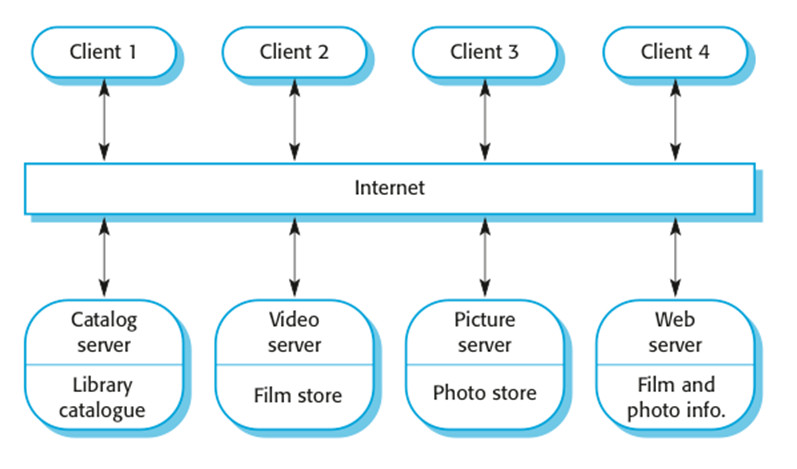
\includegraphics[scale=0.7]{architectureClientServer}
	}
	\caption{Una arquitectura cliente servidor para una filmoteca}
	\source{fuente: \cite{sommerville2011software}}
	\label{Una arquitectura cliente servidor para una filmoteca}
\end{figure}

\subsection{Patrón diseño: modelo vista controlador}

La idea de un patrón es una forma de presentar, compartir y reutilizar el
conocimiento sobre un sistema de software. Se piensa en un patrón
arquitectónico como una estilizada descripción abstracta de buena práctica,
que ha sido probada en diferentes sistemas y entornos. \cite{sommerville2011software}

En la figura \ref{fig:Arquitectura de aplicación web utilizando el patrón MVC},
se muestra una arquitectura de ejecución, cuando este patrón utiliza la
gestión en un sistema basado en la web. \cite{sommerville2011software}

\begin{minipage}{1.0\textwidth}
	\centering
	\fbox{
		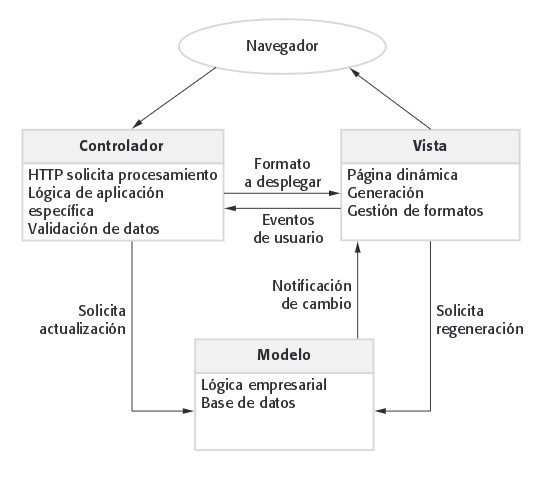
\includegraphics[scale=0.7]{mvcPattern}
	}
	\captionof{figure}{Arquitectura de aplicación web utilizando el patrón MVC}
	\source{fuente: \cite{sommerville2011software}}
	\label{fig:Arquitectura de aplicación web utilizando el patrón MVC}
\end{minipage}

\begin{itemize}

\item \textbf{Diseño del proyecto}

Se considera como patrón base de diseño Modelo Vista Controlador para realizar
la extension de funcionalidad de un Controlador representado como Administrador,
este Administrador realiza una abstracción y re uso de funcionalidad descrito
en la figura \ref{fig:Arquitectura extendida MVCA}.

\begin{minipage}{1.0\textwidth}
	\centering
	\fbox{
		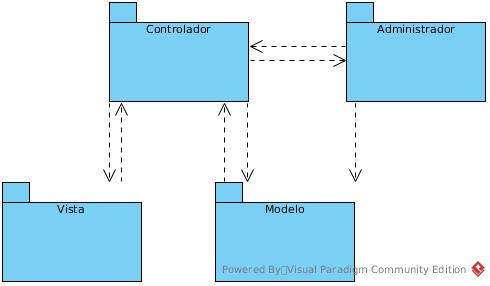
\includegraphics[scale=0.5]{mvcm}
	}
	\captionof{figure}{Arquitectura extendida MVCA}
	\source{fuente: (Elaboración propia)}
	\label{fig:Arquitectura extendida MVCA}
\end{minipage}

\end{itemize}

\section{Designación de rol}

En la plataforma web educativa se implementan cuatro tipos de roles.

\begin{itemize}

\item \textbf{Autorregulado}, rol designado a realizar suscripción o dar de
baja la misma.

\item \textbf{Tutor}, rol designado a un estudiante adscrito de la Carrera de
LAEL, quien tiene la posibilidad de crear podcast de tipo audio/vídeo, agregar
retro alimentación y agregar una transcripción. 

\item \textbf{Coordinador}, rol designado al docente de la Carrera de LAEL, quien
realiza la función de tutor y tiene la posibilidad de crear una categoría.

\item \textbf{Administrador}, rol designado a un adscrito de la Carrera de
Informática, quien tiene la posibilidad de gestionar la seguridad del sistema.

\end{itemize}

\section{Estructura de un podcast} \label{structPodcast}

Un podcast de tipo audio es representado como una estructura que contiene los
siguientes datos.

\begin{itemize}

\item \textbf{título}, nombre representativo, utilizado como identificador.
\item \textbf{imagen de portada}, imagen representativa.
\item \textbf{descripción}, resumen del tema.
\item \textbf{reproductor de audio}, grabación de diálogo.
\item \textbf{fecha de liberación}, fecha de publicación.
\item \textbf{historieta}, imagen de los personajes.
\item \textbf{transcripción}, texto del dialogo.
\item \textbf{actividad}, retro alimentación de actividad.
\item \textbf{resolución}, respuesta de actividad.
\item \textbf{glosario}, descripción de los términos.
\item \textbf{diccionario}, documento de referencia. 

\end{itemize}

Se describe la estructura de un podcast de tipo vídeo; con la diferencia de
tener: transcripción, actividad, resolución de actividad y glosario.

\begin{itemize}

\item \textbf{título}, nombre representativo, utilizado como identificador.
\item \textbf{imagen de portada}, imagen representativa.
\item \textbf{descripción}, resumen del tema.
\item \textbf{reproductor de vídeo}, uso de recursos: imagen, texto y audio.
\item \textbf{fecha liberación}, fecha de publicación.
\item \textbf{infografía}, imágenes descriptivas de tamaño pequeño.
\item \textbf{diccionario}, documento de referencia. 

\end{itemize}

\section{Definición de un componente}

Se considera el siguiente aspecto para describir el proceso de desarrollo.

\begin{itemize}

\item Tarjeta de historia de usuario.
\item Arquitectura de componente.
\item Modelo de componente.
\item Componente.
\item Implementar componente.
\item Problema/Solución de componente.

\end{itemize}

\section{\textquestiondown Cómo implementar un servicio agregado de noticia?} \label{serviceFeed}

La principal tarea de un servicio agregado de noticia es realizar la
notificación vía correo electrónico de nuevo contenido publicado en la web.

En la figura \ref{fig:Arquitectura job queue}, se muestra los componentes de
un servicio agregado de noticia y respectiva comunicación, un proceso en
segundo plano \footnote{segundo plano: Es un programa que se ejecuta sin
intervención del usuario. \cite{background}} se ejecuta respecto la fecha
de liberación descrito en la estructura de un podcast. sección
\ref{structPodcast}

\begin{minipage}{1.0\textwidth}
	\centering
	\fbox{
	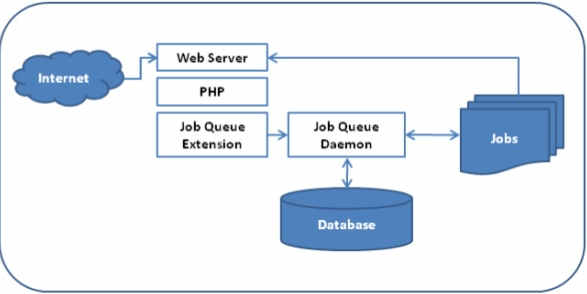
\includegraphics[scale=0.6]{jobQueue}
	}
	\captionof{figure}{Arquitectura job queue}
	\source{fuente:\cite{ossCamp2014}}
	\label{fig:Arquitectura job queue}
\end{minipage}

\subsection{Tarjeta de historia de usuario}

El equipo de informática realizó la elaboración de las historias respecto
a los deseos y sugerencias de un Coordinador de la Carrera de LAEL.

En particular deseo enfatizar los siguientes deseos a realizar:

\begin{itemize}

\item \textbf{Suscripción manual}, tabla: \ref{Tarjeta historia de usuario 03}

\end{itemize}

% add history card 03
\begin{minipage}[!htb]{\hsize}\centering
\begin{tabular}{|l|l|l|}
\hline
 & \textbf{Tarjeta Historia de Usuario} &  \\ \hline
ID Historia: 03 & \begin{tabular}[c]{@{}l@{}}Nombre: Suscripción a una\\ categoría.\end{tabular} & Fecha: 22/04/2014 \\ \hline
\multicolumn{3}{|l|}{Rol: Aprendiz autorregulado} \\ \hline
\begin{tabular}[c]{@{}l@{}}Modificación de historia\\ número: 05\end{tabular} & \begin{tabular}[c]{@{}l@{}}Iteración asignada: 7,8\end{tabular} & Prioridad en negocio: Medio \\ \hline
Tiempo estimado inicial: 20 & Riesgo en desarrollo: & Tipo de historia: Funcional \\ \hline
\multicolumn{3}{|l|}{\begin{tabular}[c]{@{}l@{}}Descripción:\\ \\ Yo como usuario aprendiz autorregulado deseo suscribirme a un determinado lenguaje \\ (francés básico, ingles básico, quechua básico, quechua psicosocial, fonética quechua), \\tal que me beneficie en recibir notificación de nuevo contenido vía correo. \\ Para esto ya no necesito ingresar mi correo electrónico.\end{tabular}} \\ \hline
\multicolumn{3}{|l|}{\begin{tabular}[c]{@{}l@{}}Pre condición:	\\ \\ Contenido publicado. \\ Servidor SMTP externo configurado.\\ Configuración de credenciales en sistema con servidor SMTP.\end{tabular}} \\ \hline
\multicolumn{3}{|l|}{\begin{tabular}[c]{@{}l@{}}Post condición:\\ \\ Recibir un mensaje en mi bandeja de entrada de mi cuenta de correo.\end{tabular}} \\ \hline
\multicolumn{3}{|l|}{\begin{tabular}[c]{@{}l@{}}Actividades:\\ \\ Desplegar lista de categorías para suscripción.\\ Permitir al usuario seleccionar de la lista de categoría para suscribirse. \\ Guardar suscripción de usuario y registrar fecha.\end{tabular}} \\ \hline
\multicolumn{3}{|l|}{\begin{tabular}[c]{@{}l@{}}Observaciones:\\ \\ La suscripción permite acceder a las noticias de nuevos contenidos de categoría.\end{tabular}} \\ \hline
\begin{tabular}[c]{@{}l@{}}.....................................................\\ Msc. Lic. Vladimir Costas Juaregui\\ PROJECT MANAGER\end{tabular} & \begin{tabular}[c]{@{}l@{}}..........................................\\ Lic. Manuel Camacho Arce\\ PRODUCT OWNER\end{tabular} & \begin{tabular}[c]{@{}l@{}}.........................................\\ Juan Omar Huanca Balboa\\ SCRUM MASTER\end{tabular} \\ \hline
\end{tabular}
\captionof{table}{Tarjeta historia de usuario 03}
\source{fuente: (Elaboración propia)}
\label{Tarjeta historia de usuario 03}
\end{minipage}

\subsection{Arquitectura de componente}

\begin{itemize}

\item \textbf{Suscripción manual}
en la figura \ref{fig:Diagrama de caso de uso registrar suscripción de usuario},
las acciones del rol autorregulado realiza el requerimiento descrito en tabla
\ref{Tarjeta historia de usuario 03}.

\begin{minipage}{1.0\textwidth}
	\centering
	\fbox{
		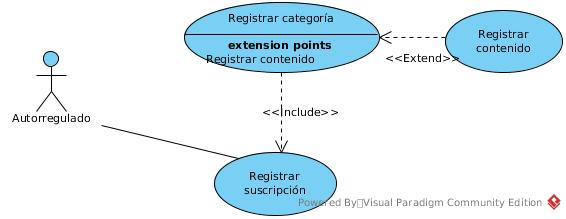
\includegraphics[scale=0.6]{useCaseRegisterSubscription}
	}
	\captionof{figure}{Diagrama de caso de uso registrar suscripción de usuario}
	\source{fuente: (Elaboración propia)}
	\label{fig:Diagrama de caso de uso registrar suscripción de usuario}
\end{minipage}

\item \textbf{Suscripción manual}
en la figura \ref{fig:Diagrama de clase para suscripción de usuario}, el diagrama
representa la composición de datos y comunicación de las clases.

\begin{minipage}{1.0\textwidth}
	\centering
	\fbox{
		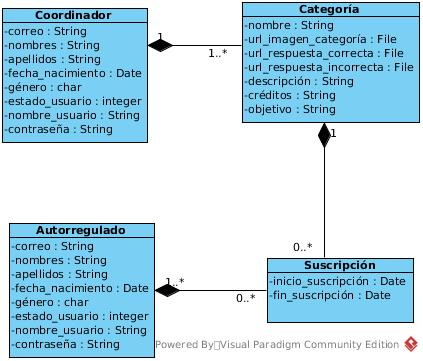
\includegraphics[scale=0.6]{classRegisterSubscription}
	}
	\captionof{figure}{Diagrama de clase para suscripción de usuario}
	\source{fuente: (Elaboración propia)}
	\label{fig:Diagrama de clase para suscripción de usuario}
\end{minipage}

\item \textbf{Suscripción manual}
en la figura \ref{fig:Diagrama de secuencia para suscripción}, el diagrama
de secuencia representa la comunicación del rol autorregulado con las
diferentes clases.

\begin{minipage}{1.0\textwidth}
	\centering
	\fbox{
		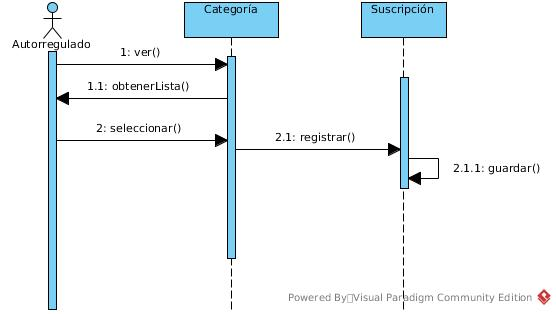
\includegraphics[scale=0.7]{sequenceRegisterSubscription}
	}
	\captionof{figure}{Diagrama de secuencia para suscripción}
	\source{fuente: (Elaboración propia)}
	\label{fig:Diagrama de secuencia para suscripción}
\end{minipage}

\end{itemize}

\subsection{Modelo de componente}

\begin{itemize}

\item \textbf{Suscripción manual} 
en la figura \ref{fig:Modelo de datos para suscripción de usuario}, el modelo de datos
representa la persistencia de suscripción de categoría y suscripción por
red social.

\begin{minipage}{1.0\textwidth}
	\centering
	\fbox{
		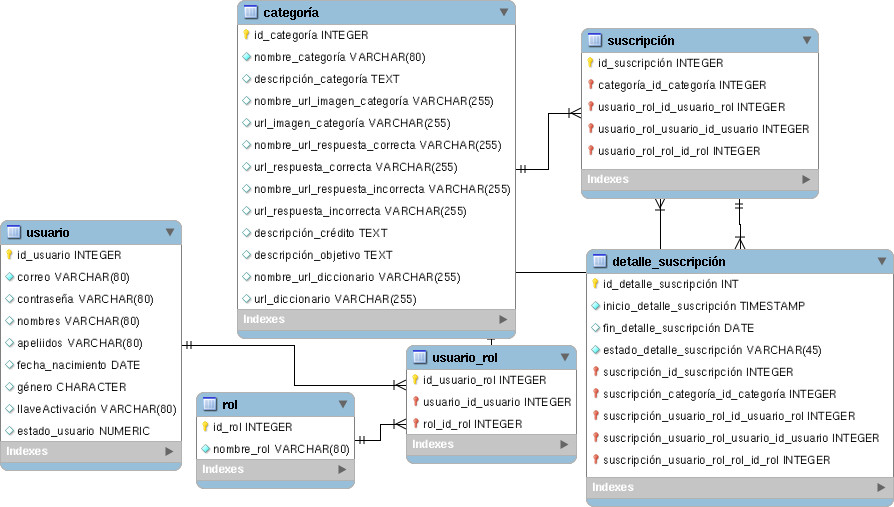
\includegraphics[scale=0.5]{modelRegisterSubscription}
	}
	\captionof{figure}{Modelo de datos para suscripción de usuario}
	\source{fuente: (Elaboración propia)}
	\label{fig:Modelo de datos para suscripción de usuario}
\end{minipage}

La suscripción conformado por categoría genera una bitácora \footnote{bitácora:
Mecanismo persistencia de actividades en el tiempo. (Elaboración propia)}
y detalle\textunderscore suscripción.

\end{itemize}

\subsection{Componente}

\begin{itemize}

\item \textbf{Suscripción}
se propone la primera opción para realizar una suscripción.

\begin{itemize}

\item \textbf{Manual}, permite realizar la suscripción con una dirección de
correo sujeto a verificación de sistema.

\end{itemize}

\textbf{Manual} en la figura \ref{fig:Ventana emergente de suscripción}, se
representa un formulario de registro de dirección de correo electrónico para
realizar una suscripción. 

\begin{minipage}{1.0\textwidth}
	\centering
	\fbox{
		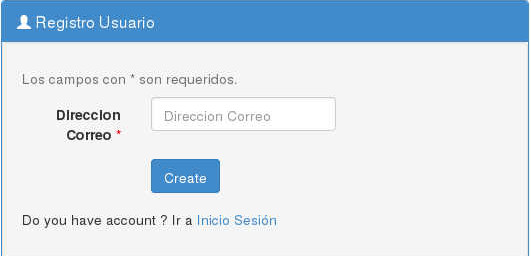
\includegraphics[scale=0.7]{modalSubscribe}
	}
	\captionof{figure}{Ventana emergente de suscripción}
	\source{fuente: (Elaboración propia)}
	\label{fig:Ventana emergente de suscripción}
\end{minipage}

\end{itemize}
	
\subsection{Implementar componente}

\begin{itemize}

\item \textbf{Suscripción - implementar en el servidor} el
siguiente segmento de código permite personalizar la suscripción por
categoría, el suscriptor obtiene las categorías habilitadas. 

\begin{lstlisting}[language=PHP, caption={Personalización de suscriptor.}]
public function actionCustomRss($idCategory) {
    ob_end_clean();
    header('Content-type: text/xml; charset=utf-8');
    $this->layout = false;    // turn off layout
    $criteria = new CDbCriteria;     // add custom criteria
    $criteria->addCondition('t.category_id_category=:Column1');
    $criteria->addCondition('t.category_id_category in (select i.category_id_category
    from interest as i) and t.content_status=' . Yii::app()->params[
    'stateContentAvailable']);
    $criteria->select = 't.title,t.summary,t.date_leave';
    $criteria->params = array(':Column1' => $idCategory);
    $data = Content::model()->findAll($criteria);
    $this->renderPartial('_viewItemChannel', array(
        'data' => $data,
    ));     // redirect view
}
\end{lstlisting}

En la linea dos tiene la funcionalidad limpiar buffer de salida y
des habilitar su uso.

En la linea tres agrega la cabecera de un documento XML y codificación con
el formato UTF-8 \footnote{UTF-8: El estándar Unicode cubre todos
los caracteres, signos de puntuación y símbolos en el mundo. Unicode 
procesamiento, almacenamiento y transporte de texto, independiente de la 
plataforma y lenguaje \cite{utf8}}.

\end{itemize}

\subsection{Problema/Solución de componente}

\begin{itemize}

\item \textbf{Suscripción manual} la dificultad surgió para implementar.

\begin{itemize}

\item Generación única de modal \footnote{modal: Una ventana modal es,
por tanto, normalmente una ventana secundaria. El usuario tiene interarticular
con el antes de que el control se pueda devolver a la solicitud principal.
\cite{modal}} para cada categoría.

\end{itemize}

La ventana modal utiliza el identificador de la categoría hija, para una lista
de categorías hijas pinchar sobre el botón de la ultima categoría realiza la
replica de identificador sobre los demás elementos.

\begin{enumerate}

\item \textbf{Generar único identificador por modal - implementar en el cliente}
como mecanismo de solución se generara un identificador conformado por
categoría padre y categoría hija.

\begin{lstlisting}[language=HTML, caption={Generador ventana modal.}]
<?php $this->beginWidget(
        'booster.widgets.TbModal', array(
    'id' => 'myModal' . $category_id,
));?>
<div class="modal-body">
    <div class="panel-body">
        <?php $this->renderPartial('//site/createRegisterSuscribe', 
        array('model_user' => $model_user)); ?>
    </div>
</div>
<?php $this->endWidget(); ?>
\end{lstlisting}

El problema de notificación vía correo electrónico se genera por las etiquetas
propias de HTML \footnote{HTML: Es el conjunto de símbolos de marcado o
códigos insertados en un archivo destinado a la visualización de una página
web mundial. \cite{html}}.

\end{enumerate}

\end{itemize}